\documentclass{article}

\usepackage{amsmath, amsthm, amssymb, amsfonts}
\usepackage{thmtools}
\usepackage{graphicx}
\usepackage{setspace}
\usepackage{geometry}
\usepackage{float}
\usepackage{hyperref}
\usepackage[utf8]{inputenc}
\usepackage[english]{babel}
\usepackage{framed}
\usepackage[dvipsnames]{xcolor}
\usepackage[most]{tcolorbox}
\usepackage{minted}
\usepackage{enumitem}
\usepackage{booktabs}
\usepackage{multirow}

\usepackage{indentfirst}

\usepackage[export]{adjustbox} % Align images

\colorlet{LightGray}{White!90!Periwinkle}
\colorlet{LightOrange}{Orange!15}
\colorlet{LightGreen}{Green!15}

\newcommand{\HRule}[1]{\rule{\linewidth}{#1}}

\newtcbtheorem[auto counter,number within=section]{code}{Código}{
  colback=LightOrange!20,
  colframe=LightOrange,
  colbacktitle=LightOrange,
  fonttitle=\bfseries\color{black},
  boxed title style={size=small,colframe=LightOrange},
}{code}

\setstretch{1.2}
\geometry{
  textheight=22.5cm,
  textwidth=13.75cm,
  top=2.5cm,
  headheight=12pt,
  headsep=25pt,
  footskip=30pt
}

% ------------------------------------------------------------------------------

\begin{document}

% ------------------------------------------------------------------------------
% Cover Page and ToC
% ------------------------------------------------------------------------------
\begin{center}
  \begin{figure}
    
\includegraphics[scale = 0.3, left]{img/IST_A.eps} % IST logo
    \end{figure}
  \LARGE{ \normalsize \textsc{} \\
  [2.0cm] 
  \LARGE{ \LARGE \textsc{Machine Learning}} \\
  [1cm]
  \LARGE{ \LARGE \textsc{LEIC IST-UL}} \\
  [1cm]
  \HRule{1.5pt} \\
  [0.4cm]
  \LARGE \textbf{\uppercase{Relatório - Homework 1}}
  \HRule{1.5pt}
  \\ [2.5cm]
  }
\end{center}

\begin{flushleft}
  \textbf{\LARGE Grupo 10:}
\end{flushleft}

\begin{center}
  \begin{minipage}{0.7\textwidth}
      \begin{flushleft}
        \large Gabriel Ferreira \\
        \large  Irell Zane
      \end{flushleft}
  \end{minipage}%
  \begin{minipage}{0.3\textwidth}
      \begin{flushright}
        \large 107030\\
        \large 107161
      \end{flushright}
  \end{minipage}
\end{center}

\begin{center}
  \vspace{4cm}
  \date \large \bf  2024/2025 -- 1st Semester, P1
\end{center}

\setcounter{page}{0}
\thispagestyle{empty}
\renewcommand{\thesection}{\Roman{section}}

\newpage

% ------------------------------------------------------------------------------
% Content
% ------------------------------------------------------------------------------



\large{\textbf{Part I}: Pen and paper}\normalsize




\begin{enumerate}[leftmargin=\labelsep]
\item Completion of the decision tree.

\hspace{3pt}

\begin{minipage}{0.4\textwidth}
  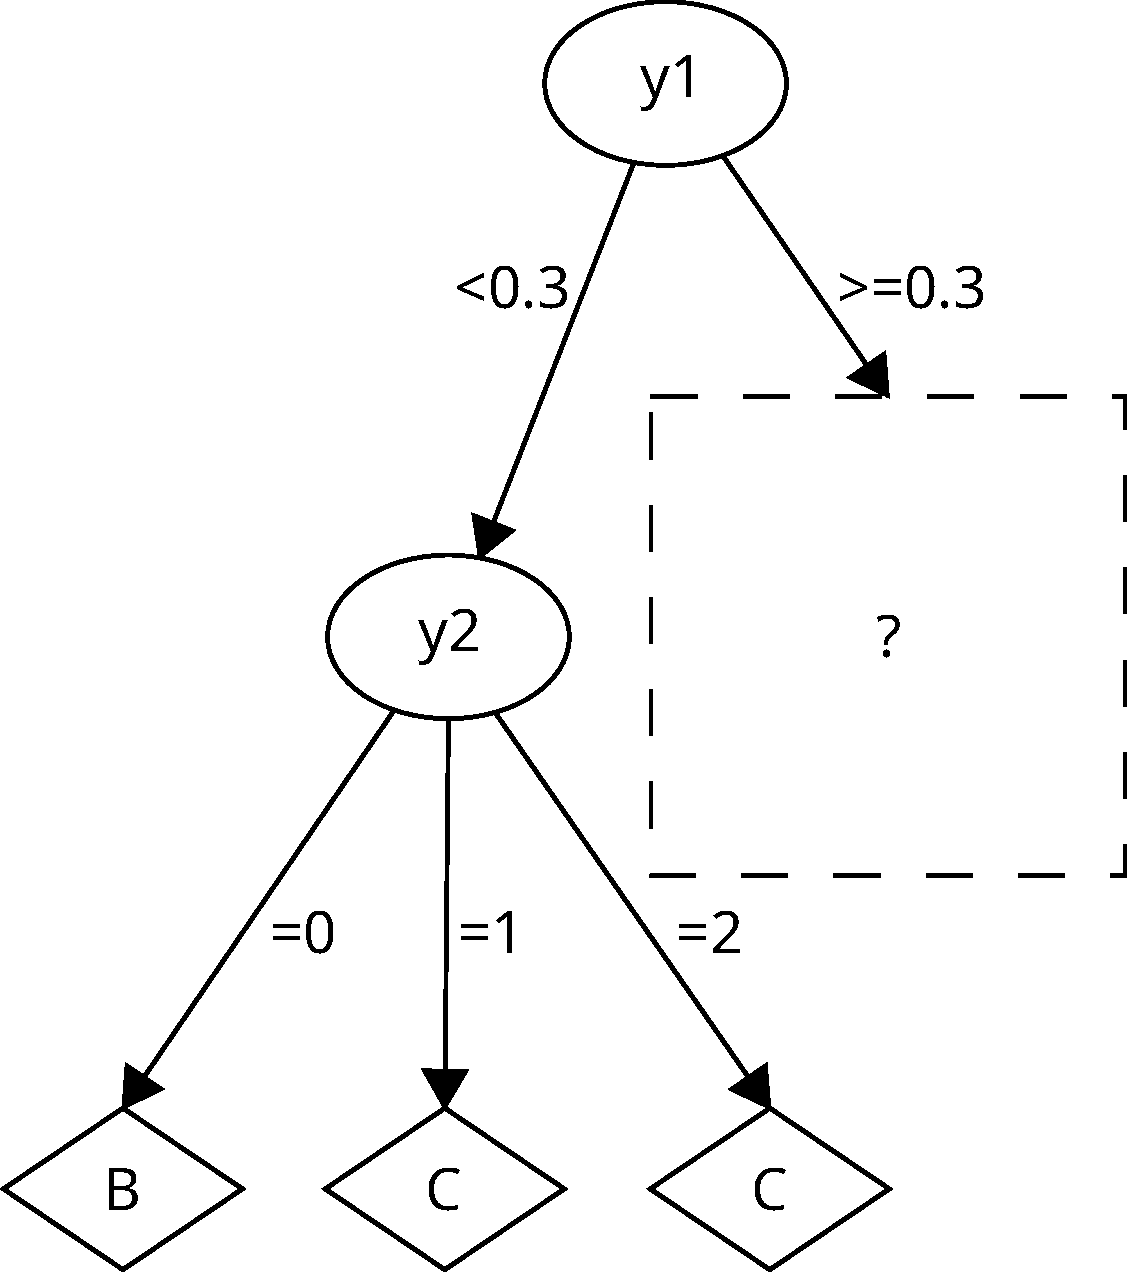
\includegraphics[scale = 0.3, left]{img/decision_tree_1.pdf}
\end{minipage}
\hspace{0.05\textwidth}
\begin{minipage}{0.6\textwidth}
  The node we must decide what to do it is on the right for 
  the dataset $D | (y1 >= 0.3)$.
  \begin{table}[H]
    \centering
    \begin{tabular}{@{}ccccc}
      $D | (y1 >= 0.3)$ & $y_2$ & $y_3$ & $y_4$ & $y_{out}$ \\ \midrule
      $x_6$  & 0 & 1 & 0 & B \\
      $x_7$  & 0 & 1 & 1 & A \\
      $x_8$  & 1 & 0 & 0 & A \\
      $x_9$  & 0 & 1 & 1 & C \\
      $x_{10}$ & 0 & 1 & 1 & C \\
      $x_{11}$ & 1 & 0 & 0 & A \\
      $x_{12}$ & 1 & 2 & 0 & B \\
    \end{tabular}
  \end{table}

  Since there are distinct $y_{out}$ values, and more 
  than 4 observations. We can split this node.
\end{minipage}
 
\hspace{3pt}

To decide the next variable to use, we must calculate 
the Information Gain of each variable using Shannon 
entropy for the dataset.

\begin{equation*}
    H(y_{out}) = -\frac{3}{7}log_2(\frac{3}{7})-\frac{2}{7}log_2(\frac{2}{7})-\frac{2}{7}log_2(\frac{2}{7}) \\ [2ex]
    = 1.57
\end{equation*}

\begin{equation*}
  H(y_{out}|y_j) = \sum{-p log_2}
\end{equation*}

\begin{equation*}
  IG(y_j) = H(y_{out}) - H(y_{out}|y_j)
\end{equation*}

\begin{table}[H]
  \begin{tabular}{cc|ccccc|cc}
  $j$ & $x$                    & $p(x)$        & $p(A | x)$   & $p(B | x)$   & $p(C | x)$   & $H(y_{out}|x)$ & $H(y_{out}|y_j)$ & $IG(y_{out}|y_j)$ \\ \midrule
  \multirow{2}{*}{2} & $y_2=0$ & $\frac{4}{7}$ & $\frac{1}{4}$ & $\frac{1}{4}$ & $\frac{2}{4}$ & 1.5  & \multirow{2}{*}{1.25} & \multirow{2}{*}{0.31} \\
   &                   $y_2=1$ & $\frac{3}{7}$ & $\frac{2}{3}$ & $\frac{1}{3}$ & $\frac{0}{3}$ & 0.92 &  &  \\ \midrule
  \multirow{3}{*}{3} & $y_3=0$ & $\frac{2}{7}$ & $\frac{2}{2}$ & $\frac{0}{2}$ & $\frac{0}{2}$ & 0    & \multirow{3}{*}{0.86} & \multirow{3}{*}{0.70} \\
   &                   $y_3=1$ & $\frac{4}{7}$ & $\frac{1}{4}$ & $\frac{1}{4}$ & $\frac{2}{4}$ & 1.5  &  &  \\
   &                   $y_3=2$ & $\frac{1}{7}$ & $\frac{0}{1}$ & $\frac{1}{1}$ & $\frac{0}{1}$ & 0    &  &  \\ \midrule
  \multirow{2}{*}{4} & $y_4=0$ & $\frac{4}{7}$ & $\frac{2}{4}$ & $\frac{2}{4}$ & $\frac{0}{4}$ & 1    & \multirow{2}{*}{0.96} & \multirow{2}{*}{0.60} \\
   &                   $y_2=4$ & $\frac{3}{7}$ & $\frac{1}{3}$ & $\frac{0}{3}$ & $\frac{2}{3}$ & 0.92 &  &  \\ \bottomrule
  \end{tabular}
\end{table}

Seeing that $y_4$ is the variable with the most information 
gain, it is the one that should be chosen to split the node.


\begin{minipage}{0.5\textwidth}
  \begin{table}[H]
    \centering
    \begin{tabular}{@{}cccc}
      $D | (y1 >= 0.3)$ & $y_2$ & $y_3$ & $y_{out}$ \\ \midrule
      $x_6$    & 0 & 1 & B \\
      $x_8$    & 1 & 0 & A \\
      $x_{11}$ & 1 & 0 & A \\
      $x_{12}$ & 1 & 2 & B \\
    \end{tabular}
  \end{table}
\end{minipage}
\begin{minipage}{0.5\textwidth}
  \begin{table}[H]
    \centering
    \begin{tabular}{@{}cccc}
      $D | (y1 >= 0.3)$ & $y_2$ & $y_3$ & $y_{out}$ \\ \midrule
      $x_7$    & 0 & 1 & A \\
      $x_9$    & 0 & 1 & C \\
      $x_{10}$ & 0 & 1 & C \\
    \end{tabular}
  \end{table}
\end{minipage}

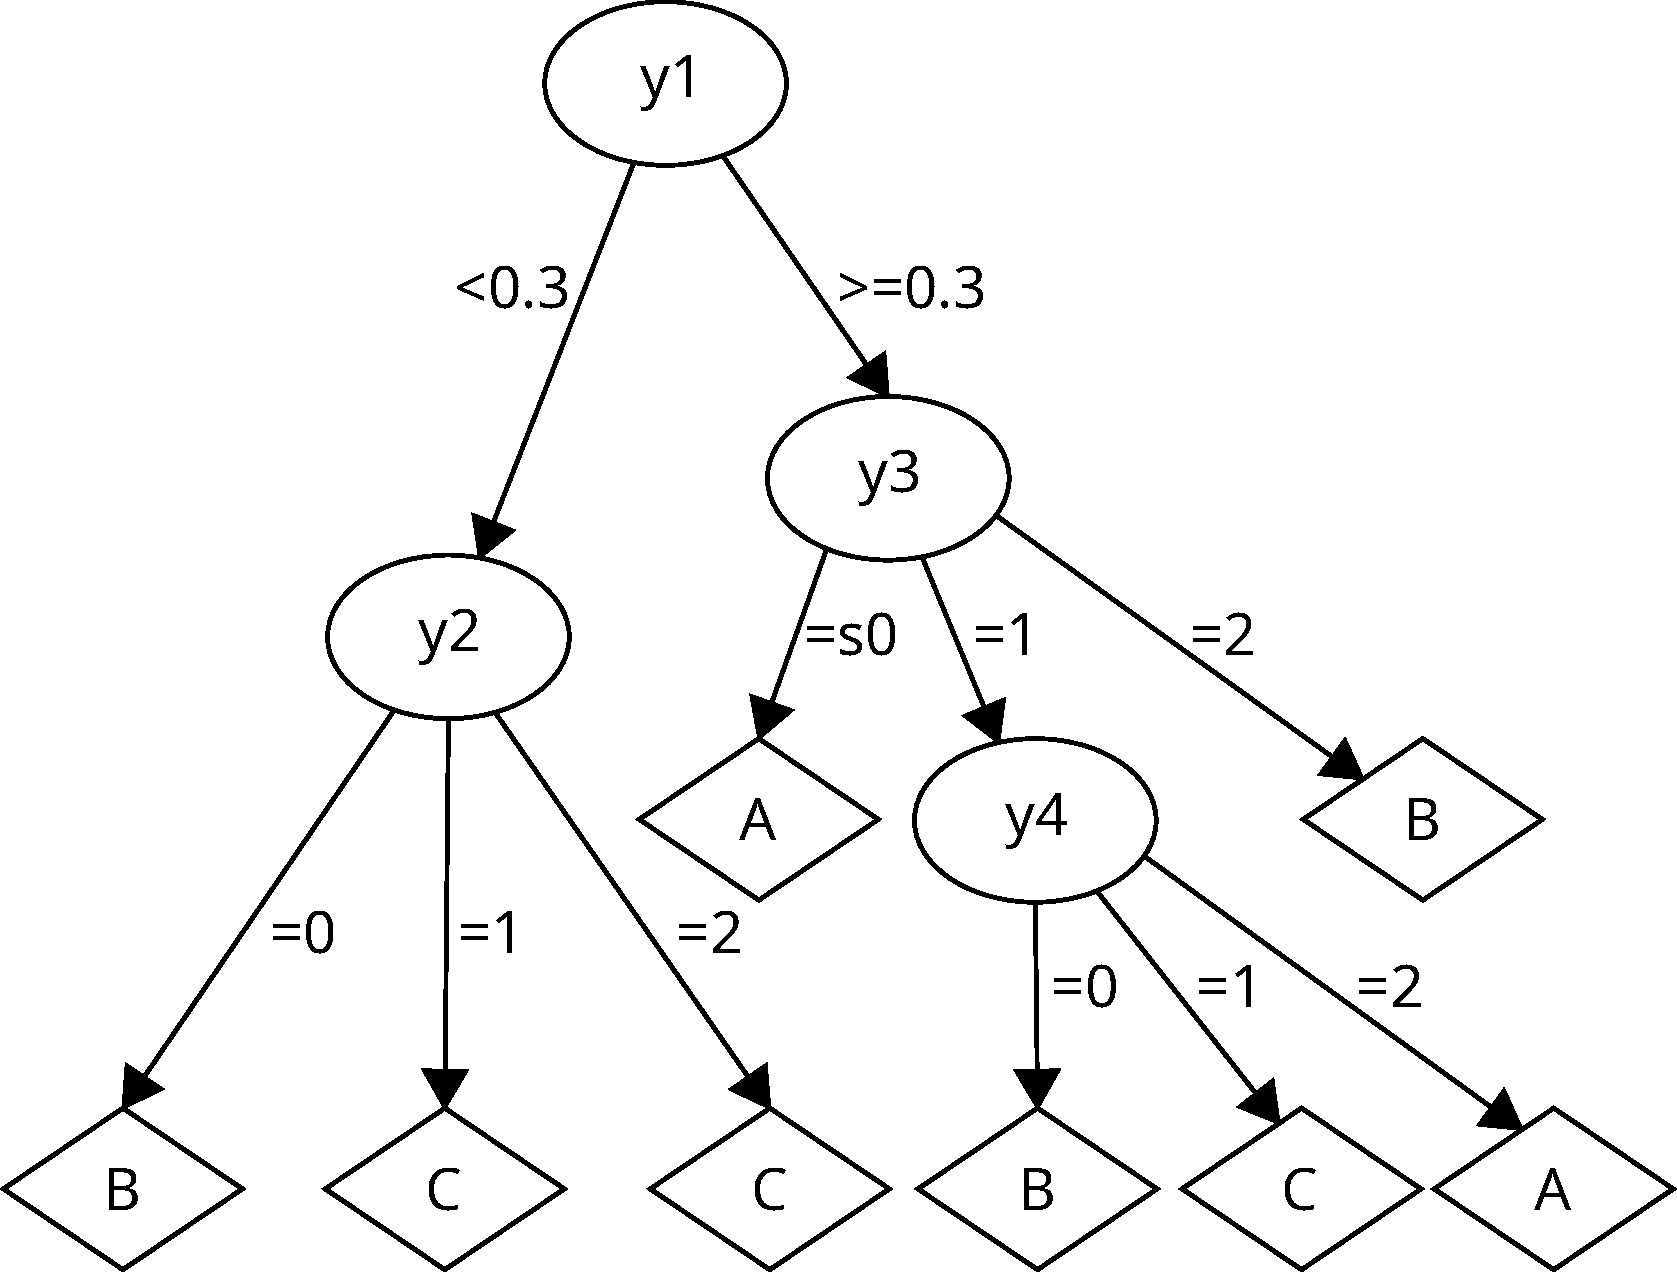
\includegraphics[scale = 0.3, left]{img/decision_tree_3.pdf}


\item Draw the confusion Matrix.


\begin{table}[H]
  \centering
  \begin{tabular}{ccccc}
      & A & B & C & \\ \midrule
    A & &&& \\
    B & &&& \\
    C & &&& \\
  \end{tabular}
\end{table}


\begin{enumerate}
\item Place your solution. Math can be entered using the equation
environment like this
\begin{equation}
    \vec{\mathbf{r}} = \vec{\mathbf{r}}_{0} + \vec{\mathbf{v}}_{0}t + \frac{1}{2}\vec{\mathbf{a}}t^{2}
\end{equation}
If you then where working in say the $x$-direction and had some numbers % A percent sign allows you to comment.
%The dollar signs around something in a line of text is for "in-line math"
\begin{equation}
\begin{array}{r@{~=~}l}
x & x_{0} + v_{x0}t + \frac{1}{2}a_{x}t^{2} \\ [2ex]
& 1.2~\text{m} + (4.0~\text{m/s})(3.0~\text{s}) + \frac{1}{2}(-1.0~\text{m/s}^{2})(3.0~\text{s})^{2}\\ [2ex]
& \boxed{8.7~\text{m}}
\end{array}
\end{equation}

\item When you get to the next part, you can add a \verb"\item" to get the appropriate label. Also,
if you don't like all the equation numbers, you can use the following to have the equation with
no number
\begin{equation*}
\sum\vec{\mathbf{F}} = m\vec{\mathbf{a}}
\end{equation*}

\item For more details on putting math into {\LaTeX} documents you can see 
\href{https://www.overleaf.com/learn/latex/Mathematical_expressions}{this page on Overleaf}.
\end{enumerate}

\item 

F1 score formula:

\[
\text{Precision} = \frac{\text{True Positives (TP)}}{\text{True Positives (TP)} + \text{False Positives (FP)}}
\]
\[
\text{Recall} = \frac{\text{True Positives (TP)}}{\text{True Positives (TP)} + \text{False Negatives (FN)}}
\]
\[
\text{F1 Score} = 2 \cdot \frac{\text{Precision} \cdot \text{Recall}}{\text{Precision} + \text{Recall}}
\]

\begin{enumerate}[label=\alph*.]

\item F1 Score for A:

\begin{itemize}
    \item True Positives (TP) = 2
    \item False Positives (FP) = 0
    \item False Negatives (FN) = 1
\end{itemize}

\[
\text{Precision}_A = \frac{2}{2 + 0} = 1
\]
\[
\text{Recall}_A = \frac{2}{2 + 1} = \frac{2}{3} \approx 0.6667
\]
\[
\text{F1}_A = 2 \cdot \frac{1 \cdot 0.6667}{1 + 0.6667} = 2 \cdot \frac{0.6667}{1.6667} \approx 0.8
\]

\item F1 Score for B:

\begin{itemize}
    \item True Positives (TP) = 4
    \item False Positives (FP) = 0
    \item False Negatives (FN) = 0
\end{itemize}

\[
\text{Precision}_B = \frac{4}{4 + 0} = 1
\]
\[
\text{Recall}_B = \frac{4}{4 + 0} = 1
\]
\[
\text{F1}_B = 2 \cdot \frac{1 \cdot 1}{1 + 1} = 1
\]

\item F1 Score for C:

\begin{itemize}
    \item True Positives (TP) = 5
    \item False Positives (FP) = 1
    \item False Negatives (FN) = 0
\end{itemize}

\[
\text{Precision}_C = \frac{5}{5 + 1} = \frac{5}{6} \approx 0.8333
\]
\[
\text{Recall}_C = \frac{5}{5 + 0} = 1
\]
\[
\text{F1}_C = 2 \cdot \frac{0.8333 \cdot 1}{0.8333 + 1} = 2 \cdot \frac{0.8333}{1.8333} \approx 0.9091
\]

\textbf{Class A has the lowest F1 Score,}
\end{enumerate}

\large{\textbf{Part II}: Programming}\normalsize

\begin{enumerate}[leftmargin=\labelsep]
\item Glucose is the feature with the best discriminative power.
Blood Pressure is the feature with the worst discriminative. power
\begin{center}
    \begin{minipage}[t]{0.45\textwidth}
        \centering
        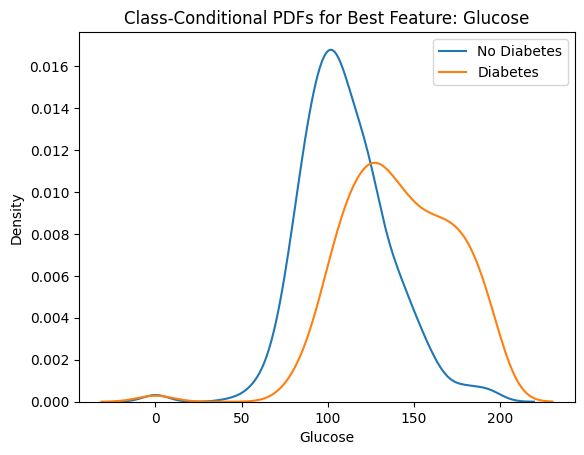
\includegraphics[width=\textwidth]{img/best_disc_feature.png} 
    \end{minipage}
    \hfill
    \begin{minipage}[t]{0.45\textwidth}
        \centering
        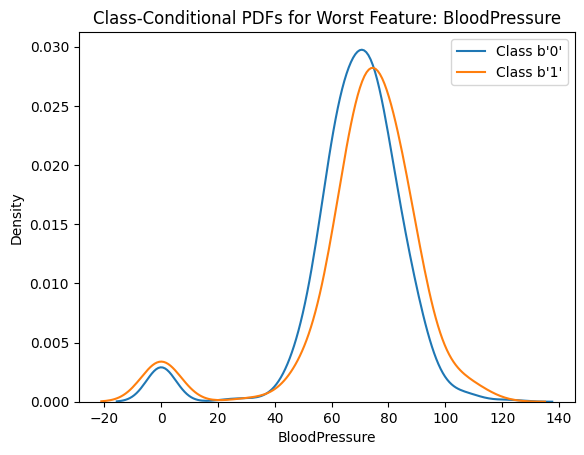
\includegraphics[width=\textwidth]{img/worst_dict_feature.png} 
    \end{minipage}
\end{center}


\item Plot of the results:
    \begin{center}
        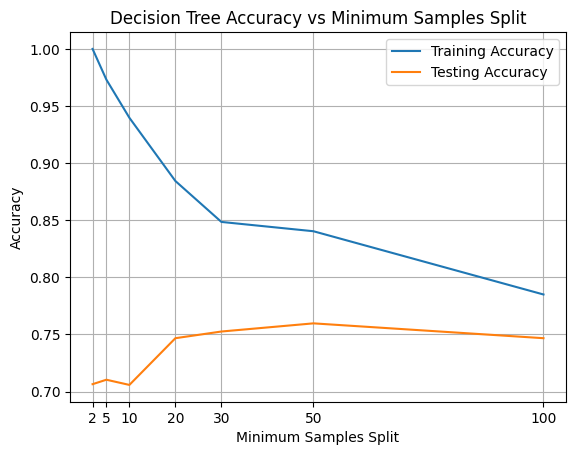
\includegraphics[width=0.5\textwidth]{img/tree_acc_vs_split.png} 
    \end{center}

\item The train accuracy decreases as the minimum samples split increases, however the test accuracies varies differently, generally increasing and then decreasing. To achieve the best generalization capacity, the minimum samples split should be set to 50, achieving a test accuracy of 76% and a train accuracy of 84%

\item Decision Tree Plot:
    \begin{center}
        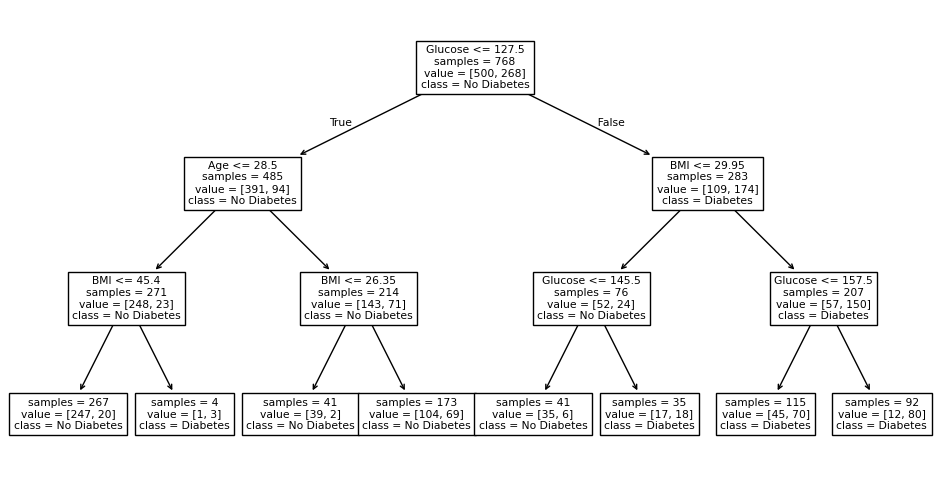
\includegraphics[width=0.9\textwidth]{img/tree_plot.png} 
    \end{center}

    \textbf{Glucose level is the primary factor}:
    \begin{itemize}
        \item If Glucose $\leq 127.5$: 18.6\% chance of diabetes
        \item If Glucose $> 127.5$: 61.6\% chance of diabetes
    \end{itemize}
    This shows that higher glucose levels are strongly associated with diabetes.

    \textbf{Age is a secondary factor for lower glucose levels}:
    \begin{itemize}
        \item If Glucose $\leq 127.5$ and Age $\leq 28.5$: 7.6\% chance of diabetes
        \item If Glucose $\leq 127.5$ and Age $> 28.5$: 32\% chance of diabetes
    \end{itemize}
    For people with lower glucose levels, being older increases the chance of diabetes.

    \textbf{BMI is important across different glucose and age ranges}:
    \begin{enumerate}[label=\alph*.]
        \item \textbf{For younger people with lower glucose}:
        \begin{itemize}
            \item If Glucose $\leq 127.5$, Age $\leq 28.5$, and BMI $\leq 45.4$: 6.7\% chance of diabetes
            \item If Glucose $\leq 127.5$, Age $\leq 28.5$, and BMI $> 45.4$: 66.7\% chance of diabetes
        \end{itemize}

        \item \textbf{For older people with lower glucose}:
        \begin{itemize}
            \item If Glucose $\leq 127.5$, Age $> 28.5$, and BMI $\leq 26.35$: 3\% chance of diabetes
            \item If Glucose $\leq 127.5$, Age $> 28.5$, and BMI $> 26.35$: 39.1\% chance of diabetes
        \end{itemize}

        \item \textbf{For people with higher glucose}:
        \begin{itemize}
            \item If Glucose $> 127.5$ and BMI $\leq 29.95$: 31.7\% chance of diabetes
            \item If Glucose $> 127.5$ and BMI $> 29.95$: 72.8\% chance of diabetes
        \end{itemize}
    \end{enumerate}
    Higher BMI is associated with a higher chance of diabetes.

    \textbf{For people with higher glucose and BMI, higher glucose levels further indicate the chance of diabetes}:
    \begin{itemize}
        \item If Glucose $> 127.5$, BMI $> 29.95$, and Glucose $\leq 154.5$: 60.9\% chance of diabetes
        \item If Glucose $> 127.5$, BMI $> 29.95$, and Glucose $> 154.5$: 85.4\% chance of diabetes
    \end{itemize}


\end{enumerate}

\vskip 1cm

\newpage

% ----------------------------------------------------------------------
% Cover
% ----------------------------------------------------------------------

\end{document}

